\documentclass{article}
\usepackage{amsmath}
\usepackage{amsfonts}
\usepackage{graphicx}
\usepackage{url}
\usepackage{float}

\author{Lucija Fekonja}
\title{Projektna naloga iz matematičnega modeliranja}

\newcommand{\R}{\mathbb{R}}
\newcommand{\N}{\mathbb N}
\newcommand{\Z}{\mathbb Z}
\newcommand{\C}{\mathbb C}
\newcommand{\Q}{\mathbb Q}



% Še neke ostale stvari ...


\begin{document}

\maketitle

Narisati želimo lik, ki nastane, ko poligonska črta prvič seka samo sebe. 
Program bo naključno izbiral točke 
in na vsakem koraku preveril ali na novo narisana daljica seka poligonsko
črto, katere del je tudi sama. Program se konča, ko najde presečišče. Tedaj 
mora le še preveriti kakšen lik se je tvoril in izračunati njegovo površino.

Naključne točke program izbira na dva načina. V prvem uporabnik določi območje 
$I \times J$, nakar program na vsakem koraku izbere točko iz tega območja. V 
drugem primeru lahko uporabnik določi tudi dolžine daljic poligonske črte. Tedaj 
bo program prvo točko izbral iz predpisanega območja $I\times J$, vsako nadaljno
pa tako, da bo njena razdalja od prejšnje tolikšna, kot jo je določil uporabnik.
Če v tem primeru
program ne najde samopresečišča, saj mu pred tem zmanjka predpisanih dolžin v seznamu 
$L$, vrne napako in izvajanje se zaključi. 
Prvi način izbire 
naključnih točk je izpisan v \path{rand_tocke.m}, drugi način pa v 
\path{rand_tocka_na_dolzini.m}. Program \path{daljica.m} riše daljice, ki povezujejo
zaporedoma izbrane točke.

Recimo, da smo narisali $n$ daljic. Označimo jih s $p_1 \dots p_{n-1}$, kjer je bila $p_1$ narisana 
prva, $p_{n-1}$ pa zadnja. Preveriti želimo, če na novo narisana daljica $p_{n-1}$ seka katero od prejšnjih.
Če sta $(x_1, y_1)$ in $(x_2, y_2)$ točki, ki ju daljica $d$ povezuje, 
potem lahko $d$ parametriziramo s parametrizacijo 
$$ d \colon (t) \mapsto ( x_1 (1 - t) + x_2 t, \; y_1 (1 - t) + y_2 t) \text{.}$$
Predstavljamo si lahko, da se točka $t$ premika v ravni črti od $(x_1, y_1)$ do 
$(x_2, y_2)$. Zato lahko, če obstaja več presečišč, opredelimo katero daljico nova 
daljica $p_{n-1}$ seka najprej, katero seka drugo itd. Dve daljici $d_1(t) = (x_1 (t), y_1 (t))$
in $d_2(t) = (x_2 (t), y_2 (t))$ se sekata, če obstajata taka $t_1$ in $t_2$, 
da je 
\begin{equation} \label{sistem}
    (x_1 (t_1), y_1 (t_1)) = (x_2 (t_2), y_2 (t_2)) \text{.}
\end{equation}
Rešujemo torej sistem
enačb z dvema neznankama, ki ima natanko eno rešitev $(t_1, t_2)$. V kolikor sta oba 
$t_1$ in $t_2$ med vključno $0$ in $1$, je rešitev veljavna, kar pomeni, da obstaja presečišče 
daljic. Na tem mestu je vredno omeniti, da imata dve zaporedoma narisani daljici v poligonski
črti vedno skupno presečišče, zato preverjamo presečišča $p_{n-1}$ zgolj z daljicami $p_1 \dots p_{n-3}$.

Vendar pa ta metoda ne deluje 
dobro kadar sta daljici vzporedni, zato predstavimo še drugo metodo s pomočjo orientacije treh točk.
V splošnem se premici doloženi z mejnima točkama 
$$ d1 = (p1, p2) \qquad d2 = (t1, t2)$$
sekata, kadar sta orientaciji trikotnikov z ogljišči $(p1, p2, t1)$ in $(p1, p2, t2)$ različni. 
Enakovredno je preverjati različnost orientacij trikotnikov $(t1, t2, p1)$ in $(t1, t2, p2)$. 
Nekoliko posebnejši primer je, ko so $p1, p2$ in $t1$ kolinearne, $t2$ pa leži med $p1$ in $p2$.
Analogno za ostale primere grupiranja točk.
\begin{figure}[H]
    \centering
    \begin{minipage}{.5\textwidth}
        \centering
        \includegraphics[height = 3cm]{splosno_sekata.eps}
        \caption{Splošen primer.}
    \end{minipage}%
    \begin{minipage}{.5\textwidth}
        \centering
        \includegraphics[height = 3cm]{kolinearne.eps}
        \caption{Poseben primer.}
        \label{fig:napih}
    \end{minipage}
\end{figure}
Orientacijo trikotnika lahko izračunamo direktno iz njegovih ogljišč. Če imamo dane točke $A = (x_1, y_1)$,
$B = (x_2, y_2)$ in $C = (x_3, y_3)$, je strmina daljice med $A$ in $B$ enaka 
$$k_1 = \frac{y_2 - y_1}{x_2 - x_1}\text{,}$$ 
strmina daljice med $B$ in $C$ pa
$$k_2 = \frac{y_3 - y_2}{x_3 - x_2}\text{.}$$
Orientacija točk je potem odvisna od $k_1 - k_2$ oz. od $(y_2 - y_1) (x_3 - x_2) - (y_3 - y_2) (x_2 - x_1)$,
kar je lahko pozitivno, negativno ali enako $0$. Če je  $k_1 = k_2$, so točke kolinearne,
če je $k_1 < k_2$, so orientirane v pozitivni smeri, t.j. v nasprotni smeri urinega kazalca, če pa
je $k_1 > k_2$, pa so orientirane v negativni smeri. V datoteki \path{preveri_presecisca_orientacija.m} 
s tem pristopom preverimo, ali se dani daljici sekata.
Šele ko vemo, če se sekata, izračunamo njuno presečišče, kar pa lahko storimo z reševanjem 
sistema enačb (\ref{sistem}). Slednje je izpisano v \path{presecisce_daljic.m}.

Takšen algoritem ima zahtevnost $O(n^2)$, saj za vsako daljico preverjamo, če se seka s katerokoli 
drugo že narisano. Boljši algoritem za iskanje presečišč $n$ premic je Bently--Ottmannov algoritem,
ki ima časovno zahtevnost $O ((n + k) \log n)$, kjer je $n$ število mejnih točk daljic, $k$ pa število 
presečišč. 

Naj bo sedaj $n$ korak, v katerem se daljice prvič sekajo. Tedaj smo narisali točke $(x_1, y_1) \dots (x_n, y_n)$
in daljice $p_1 \dots p_{n-1}$.
Spomnimo se, da ima daljica, ki povezuje točki $(x_{n-1}, y_{n-1})$ in $(x_n, y_n)$, parametrizacijo
$$ p_{n-1} (t) \mapsto ( x_{n-1} (1 - t) + x_n t, \; y_{n-1} (1 - t) + y_n t) \text{,}$$
kjer $t$ teče od točke $(x_1, y_1)$ do $(x_2, y_2)$. Zato lahko tvorimo zaporedje daljic, ki jih $p_{n-1}$ seka.
Označimo jih s $q_1 \dots q_k$, kjer je parameter $t$ v parametrizaciji $p_{n-1} (t)$ najmanjši v presečišču s $q_1$
in največji v presečišču s $q_k$.

V nadaljevanju smo iskali lik, ki nastane, ko se narisana poligonska črta prvič zapre. 
Lik je sestavljen iz točk, ki jih je program izbiral naključno in iz presečišč, ki smo jih poiskali.

Če vidimo, da je presečišče le eno, in sicer s $k$-to narisano premico, so ogljišča iskanega lika najdeno presečišče 
in točke $(x_{k+1}, y_{k+1}) \dots (x_{n-1}, y_{n-1})$. Na naslednji sliki šestata narisana daljica seka prvo, zato
za ogljišča vzamemo $(x_2, y_2) \dots (x_6, y_6)$ ter samopresečišče.
\begin{figure}[H]
    \centering
        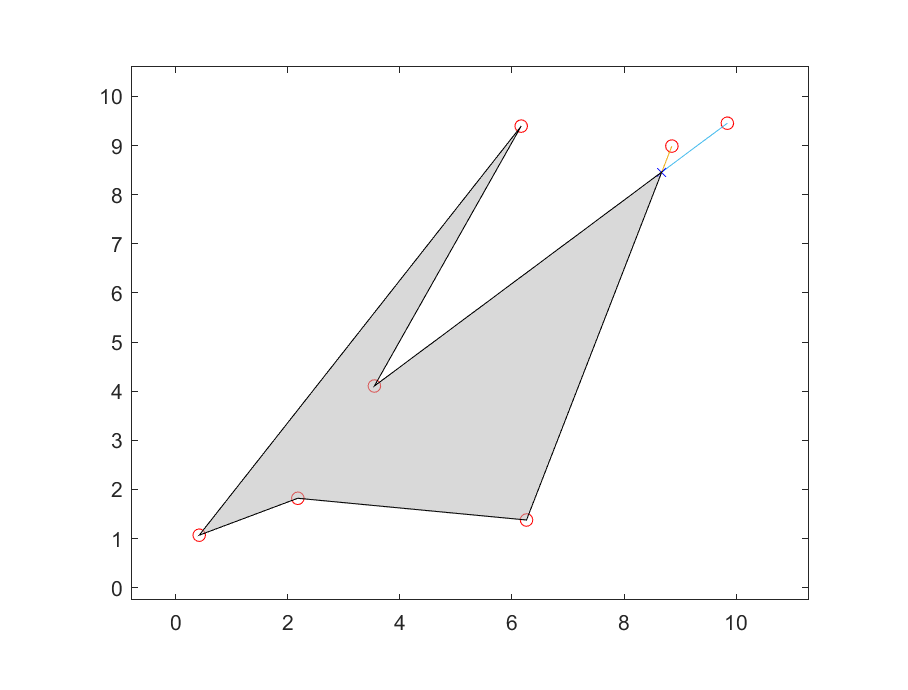
\includegraphics[height = 6cm]{eno_presecisce.eps}
        \caption{Poligonska črta z enim samopresečiščem.}
\end{figure}

V primeru, ko je presečišč več, imamo par posebnih primerov, ki jih moramo obravnavati pred splošnim. Če je bila daljica,
ki jo $p_{n-1}$ seka najprej, narisana najkasneje, naj bo to daljica $q_1 = p_i$, potem so ogljišča iskanega lika 
$(x_{i+1}, y_{i+1}) \dots (x_{n-1}, y_{n-1})$.
\begin{figure}[H]
    \centering
        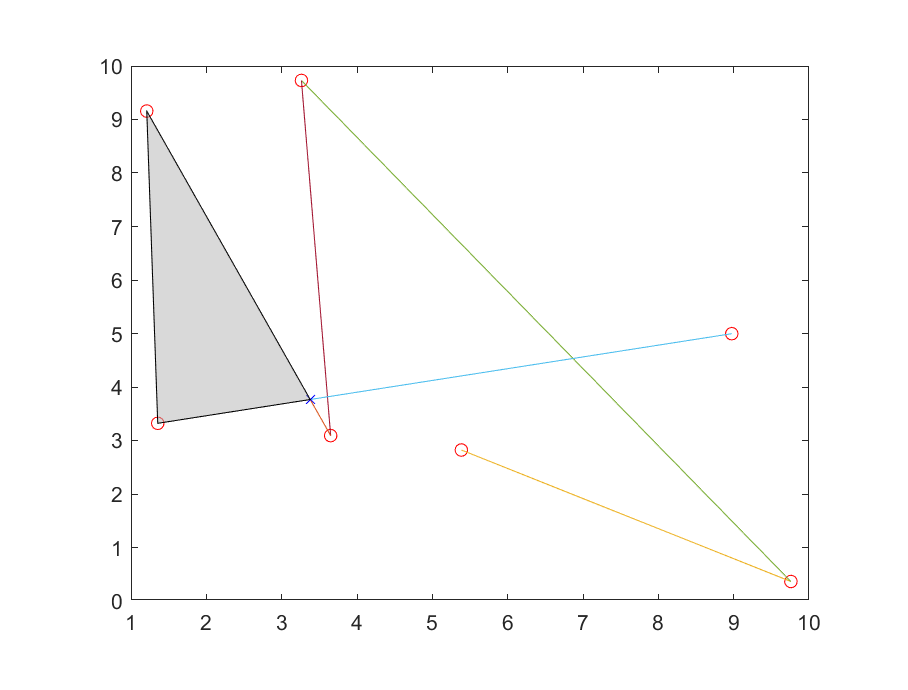
\includegraphics[height = 6cm]{k_max.eps}
        \caption{Poligonska črta, ki najprej seka nazadnje narisano črto.}
\end{figure}

Podobno velja, če je $q_1 = p_i$ bila narisana najprej, $q_2 = p_j$ pa najkasneje izmed vseh $q_1 \dots q_k$. V tem primeru 
nobena od premic $p_1 \dots p_{i-1}$ ne seka $p_{n-1}$, zato s $p_{n-1}$ ne tvorijo zaprtega lika. Ogljišča lika, ki ga iščemo 
so potem $(x_{j+1}, y_{j+1}) \dots (x_{n-1}, y_{n-1})$ ter presečišče med $q_2$ in $p_{n-1}$. Vendar pa se ta primer obdrži le,
če dobena od točk $(x_{i+1}, y_{i+1}) \dots (x_{j-1}, y_{j-1})$ ne leži znotraj tega lika. Tak primer je prikazan na naslednji
sliki. 
\begin{figure}[H]
    \centering
        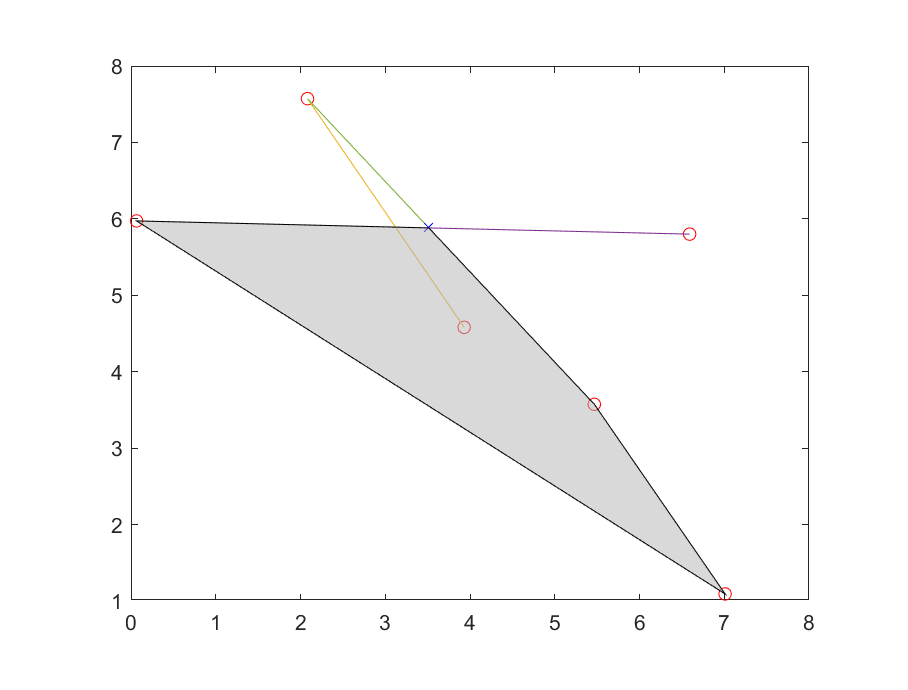
\includegraphics[height = 6cm]{ni_tocke_v_test.eps}
        \caption{Poligonska črta, ki najprej seka $q_1$, nato pa nazadnje narisano črto.}
\end{figure}

Primer, v katerem je bila $q_1 = p_i$ bila narisana najprej, $q_2 = p_j$ pa najkasneje izmed vseh $q_1 \dots q_k$, ampak 
zgornja rešitev ne bo pravilna je prikazan na naslenji sliki.
\begin{figure}[H]
    \centering
        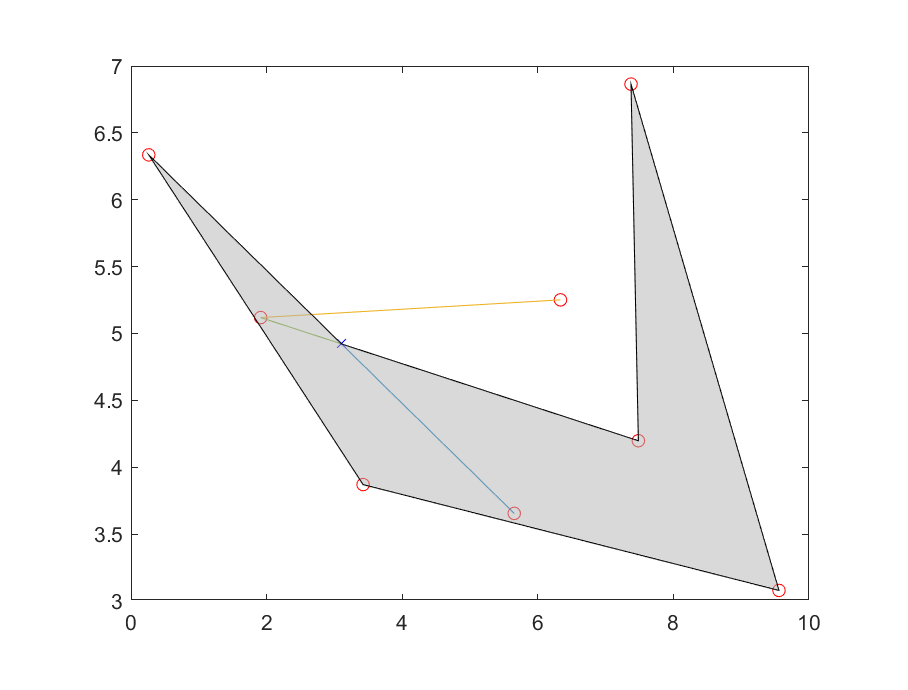
\includegraphics[height = 6cm]{tocke_v_testu.eps}
        \caption{Napačna izbira lika.}
\end{figure}

V zgornjem primeru, kot tudi vseh ostalih sledimo naslednji proceduri.
Naj bo $q_1 = p_i$ daljica, ki jo $p_{n-1}$ seka najprej, torej pri najmanjšem parametru $t$,
$q_2 = p_j$ pa pri drugem najmanjšem $t$. Daljici $q_1$ in $q_2$ v Matlabu najdemo tako, da pri iskanju presečišč
shranjujemo tudi vrednosti spremenljivke, po kateri je parametrizirana $p_{n-1}$ $t \in [0, 1]$, v katerih ima $p_{n-1}$ 
presečišče. Prav tako v to tabelo shranimo, s katero premico se $p_{n-1}$ seka. Tabelo presečišč nato uredimo po 
naraščajočem $t$ in za presečišči s $q_1$ in $q_2$ vzamemo prva dva stolpca. Nato za vse premice $p_{i+1} \dots p_{j-1}$, ki so 
bile narisane med $q_1$ in $q_2$ preverimo, če katera seka $p_{n-1}$. Če je nobena ne seka, za ogljišča iskanega lika vzamemo
presečišči $p_{n-1}$ s $q_1$ in $q_2$, ter točke $(x_{i+1}, y_{i+1}) \dots (x_{j-1}, y_{j-1})$. Naslednja slika prikazuje 
tak primer.
\begin{figure}[H]
    \centering
        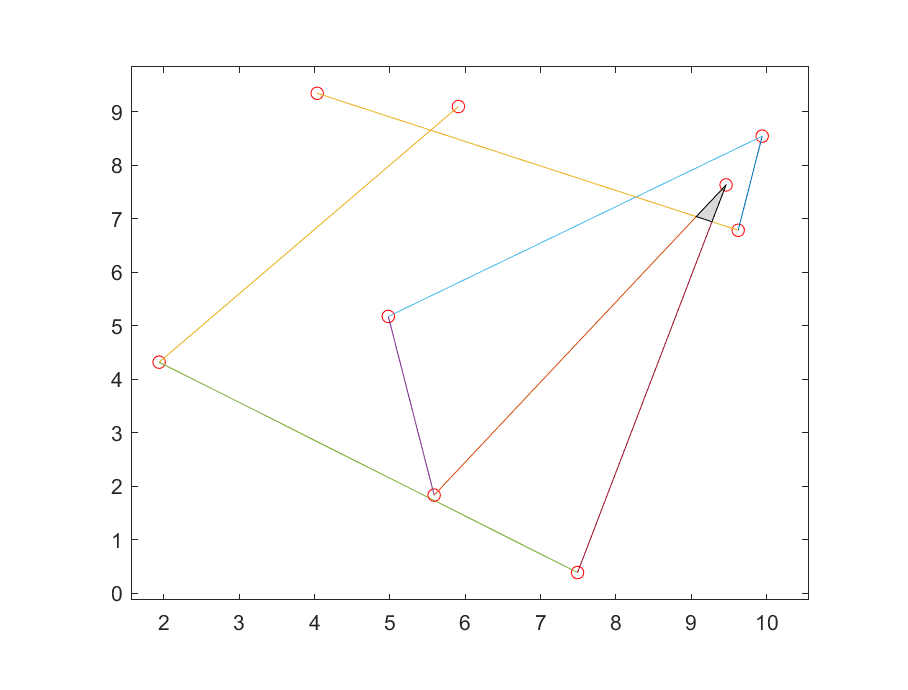
\includegraphics[height = 6cm]{zaporednje_q.eps}
        \caption{Poligonska črta, ki seka najprej tretjo in nato četrto daljico.}
\end{figure}
Če katera od daljic $p_{i+1} \dots p_{j-1}$ seka $p_{n-1}$, postopek ponovimo za $q_2$ in $q_3$. Število korakov je 
končno, saj je število presečišč končno. Ker je poligonska črta zvezna, zagotovo najdemo rešitev.

Na koncu še izračunamo ploščino lika, ki se tvori, kar najelegantneje naredimo z ukazom polyarea.

Do zdaj smo iskali le enostavne mnogokotnike. To so takšni liki, katerih stranice se ne sekajo. V splošnem lahko 
poligon seka samega sebe, zato bomo v nadaljevanju poiskali še te. Natančneje, poiskali bomo najbolj zunanji poligon,
ki omejuje neko območje. Presečišča poiščemo na isti način kot zgoraj. 
Prav tako na isti način kot prej ravnamo, če je presečišče le eno. Razlike med programi nastanejo, ko je 
presečišč več.
Lik bomo gradili postopoma in sicer iz enostavnih mnogokotnikov.

Ponovno označimo daljice, ki jih $p_{n-1}$ seka po vrsti s $q_1 \dots q_k$. 
Izmed teh daljic poiščimo tisto, ki je bila narisana zadnja. Naj bo to $q_z = p_i$.
Sedaj smo našli prvi del iskanega lika. Zanj vzemimo točke $(x_{i+1}, y_{i+1}) \dots 
(x_{n-1}, y_{n-1})$. V nadaljevanju se bom na ta lik sklicevala z lik2.

\begin{figure}[H]
    \centering
        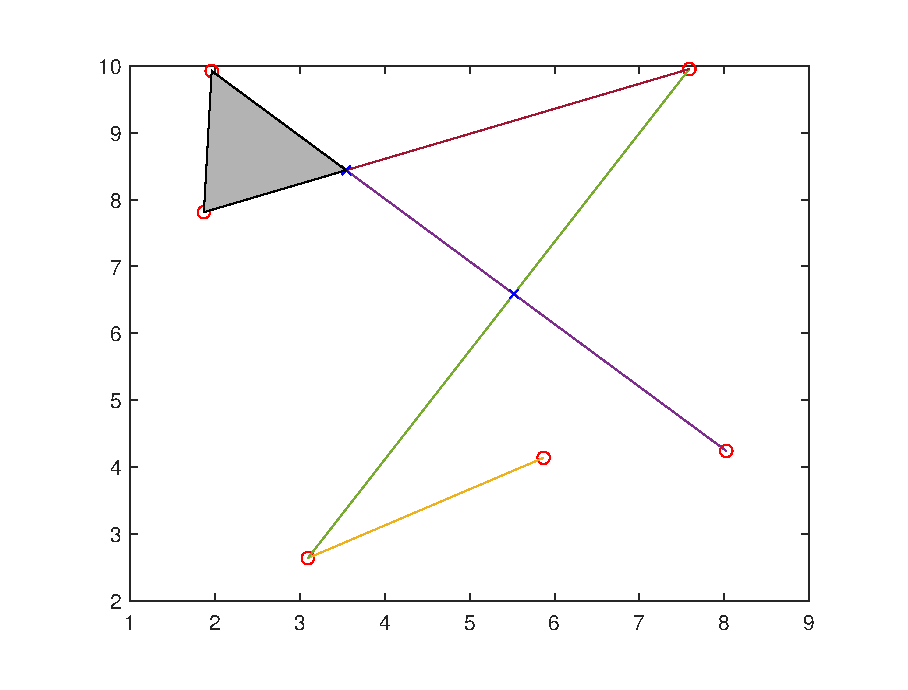
\includegraphics[height = 6cm]{del.eps}
        \caption{Obarvan prvi del iskanega lika.}
\end{figure}

Sedaj ločimo dve možnosti, saj je lahko indeks daljice $p_{p} = q_1$ manjši ali večji od indeksa daljice 
$p_{z} = q_k$. V obeh primerih poiščemo premico, ki jo $p_n$ seka za $p_{p}$. Naj bo to $p_t$.
Če je $p \; < \; z$, preverimo, če je $t > p$ in $t \leq z$. Če je, dodamo v lik vse točke
med $(x_{p + 1}, y_{p+1}) \dots (x_t, y_t)$, ki ne ležijo znotraj lika lik2 ter presečišče med $p_t$ in $p_n$.

\begin{figure}[H]
    \centering
        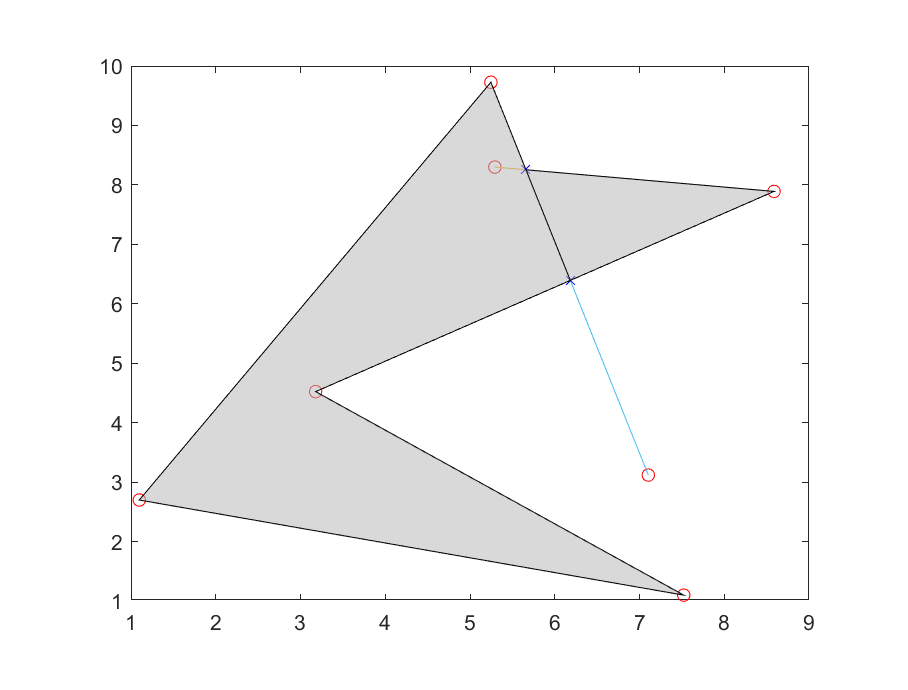
\includegraphics[height = 6cm]{seka3.eps}
        \caption{Največji lik, ki ga tvori poligonska črta, v katerem je $p < z$.}
\end{figure}

Če je $p \; > \; z$, preverimo, če je $t < p$ in $t \geq z$. Če je, dodamo v lik vse točke
med $(x_{p}, y_{p}) \dots (x_{t+1}, y_{t+1})$, ki ne ležijo znotraj lika lik2 ter presečišče med $p_t$ in $p_n$.
Končni lik dobimo, ko se sprehodimo po vseh presečiščih in vanj dodamo še lik2.

\begin{figure}[H]
    \centering
        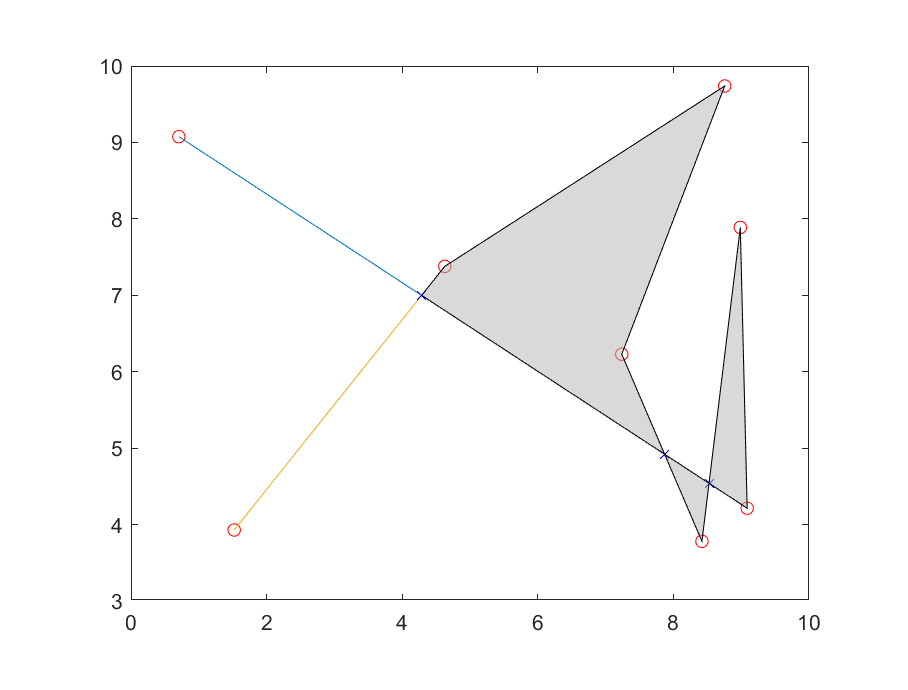
\includegraphics[height = 6cm]{seka2.eps}
        \caption{Največji lik, ki ga tvori poligonska črta, v katerem je $p > z$.}
\end{figure}



\section*{Literatura}

S. Babu, \emph{Orientation of three ordered points}, dostopno na https://iq.opengenus.org/orientation-of-three-ordered-points/

SaturnCloud, \emph{Implementing the Bentley-Ottmann Algorithm: A Comprehensive Guide}, dostopno na https://saturncloud.io/blog/implementing-the-bentleyottmann-algorithm-a-comprehensive-guide/

A. Margalit, G. D. Knott, \emph{An algorithm for computing the union, intersection or difference of two polygons}, dostopno na https://www.sciencedirect.com/science/article/abs/pii/0097849389900599


\end{document}